\scanpage{65}
(iso dans cat. dérivée) puisque $\mathbb{C}^{\bullet}$ est une résolution $\Sigma$-injective de $\Psi^0$.

\figure{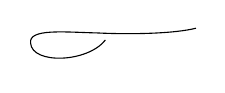
\begin{tikzpicture}[x=1cm,y=1cm]\draw (0.75,0.02) .. controls (0.52,-0.27) and (-0.18,-0.29) .. (-0.2,-0.02) .. controls (-0.23,0.17) and (0.23,0.12) .. (0.65,0.11) .. controls (1.07,0.09) and (1.62,0.1) .. (1.9,0.17);\end{tikzpicture}}

Nous considérons maintenant les réalisations $\frac12$ simpliciales $P_*\supset Q_*\supset \deleted{\unsure{Q}}P_{0*}\supset \mathbb{K}_*$ \deleted{\unsure{$Q$}} de $P\supset Q\supset \deleted{\unsure{Q}}P_0\supset\mathbb{K}$. Or sur \deleted{\unsure{la}} $P_*$ il y a la structure $\otimes_{\deleted{\unsure{\Sigma}}*}$ ou $\otimes_*$ ($L_*\otimes_*M_*$ défini \unsure{composantes par composantes|composante par composante}
\[
(L_*\otimes M_*)_{[n]}=L_{[n]}\otimes M_{[n]}\qquad)
\]
avec contraintes d'ass, unité ($\Psi^0$), et de comm., \inserted{$\otimes$ du bilex.} \deleted{\unsure{De même que la réalisation (contravariante) $P^*,Q^{\bullet}$,|De même que la réalisation (contravariante) $P^*,Q^*$,}} On note que $\mathbb{K}_*$ est un ``idéal'', i.e. que \deleted{\unsure{l'on est un des facteurs}} \inserted{\unsure{lire|i.e.}} si un des facteurs $L_*,M_*$ est dans $\mathbb{K}_*$, l'autre aussi), $P_0$ et $Q$ sont stables par $\otimes$, car
% slanted
\margin{\deleted{\unsure{et}} il n'y a pas de \uline{Hom} interne mais on a \unsure{certaines (dualités)|aussi un (des Ext)}}
\[
\begin{aligned}
\Psi^0_{\unsure{\bullet|0}*}\otimes\Psi^0_{\bullet*}&\simeq\Psi^0_{\bullet*}\quad(\Rightarrow\text{ stabilité de }\unsure{\mathcal G|\mathbb{K}|P_0})\\[-.3ex]
\underset{\mathbb 1_*}{\Vert}\hspace{1.7em}\underset{1_*}{\Vert}&\hspace{1em}\underset{\mathbb 1_*}{\Vert}
\end{aligned}
\]
et
\[
\begin{aligned}
\Psi^i_*\otimes\Psi^j_*&\simeq\Psi^{i+j}_*+\text{ élément de }\mathbb{K}\\
&(\Rightarrow\text{ stabilité de }P_{1*}=\unsure{Q'|Q})
\end{aligned}
\]

On transporte cette structure multiplicative sur $P$ et ses sous-catégories (notation $*$, pour éviter des confusions) et ses autres réalisations $P_{\bullet}$ et $P^{*}$, $P^{\bullet}$ (ces deux dernières \unsure{contragrédientes|contravariantes}). On note $*$ sur $P_{\bullet}$ et $P^{\bullet}$, et $\otimes$ ou $\overset{*}{\otimes}$ sur $P^{*}$, car l'équivalence des
% archive sheet number: 64
